\section{Additional details}

\begin{frame}{General Dirichlet boundary conditions}
	\appendixtarget{bc}
	\textbf{Problem:} $u=g$ on $\Gamma$, with $u_\theta$ the PINN prior.

	\vspace{6pt}
	\textbf{Additive approach:}
	\vspace{-3pt}
	\[
		p_h^+=g-u_\theta \quad\text{on } \Gamma.
	\]
	\vspace{-14pt}

	Homogeneous as soon as $u_\theta$ is exact on $\Gamma$ (\coloredonly<1>{exact BC in the PINN}).

	\vspace{6pt}
	\textbf{Multiplicative approach} ($u_{h,\theta}^\times=u_{\theta,M}\,p_h^\times-M$, $u_{\theta,M}=u_\theta+M$):
	\vspace{-3pt}
	\begin{align*}
		\text{standard PINN:} \quad      & p_h^\times=\frac{g+M}{u_{\theta,M}} \quad\text{on } \Gamma, \\
		\text{PINN with exact BC:} \quad & p_h^\times=1 \quad\text{on } \Gamma.
	\end{align*}
	\vspace{-14pt}

	Homogeneous case: $M=0$ possible, $p_h^\times$ left free (\coloredonly<1>{more freedom} for the derivatives at the boundary).

	\vspace{6pt}
	\textbf{Curved boundaries} (disk, $k>2$): the prior is not exact on $\partial\Omega_h$; in the tests, $g=u$ on $\partial\Omega_h$.
\end{frame}

\begin{frame}{Multiplicative gain constants}
	\appendixtarget{gain}
	\textbf{Additive:}
	\vspace{-3pt}
	\[
		C_{\text{gain}}^{+}=\frac{| u-u_{\theta} |_{H^{s+1}}}{| u |_{H^{s+1}}}
	\]
	\vspace{-4pt}

	\textbf{Multiplicative} ($1\leqslant s\leqslant k$, $s=k$ in the main slides):
	\vspace{-3pt}
	\begin{align*}
		C_{\text{gain},H^1}^{\times,M} & = \left| \frac{u_M}{u_{\theta,M}} \right|_{H^{s+1}} \frac{\| u_{\theta,M}\|_{W^{1,\infty}}}{| u |_{H^{s+1}}}, \\
		C_{\text{gain},L^2}^{\times,M} & = C_{\theta,M}\left| \frac{u_M}{u_{\theta,M}} \right|_{H^{s+1}} \frac{\| u_{\theta,M}\|_{W^{1,\infty}}^2}{| u |_{H^{s+1}}},
	\end{align*}
	\vspace{-14pt}

	\[
		C_{\theta,M}=\|u_{\theta,M}^{-1}\|_{L^{\infty}}+2|u_{\theta,M}^{-1}|_{W^{1,\infty}}+|u_{\theta,M}^{-1}|_{W^{2,\infty}}.
	\]
	\vspace{-14pt}

	\textbf{Limit:} $C_{\text{gain},H^1}^{\times,M}$ and $C_{\text{gain},L^2}^{\times,M}$ $\underset{M\to\infty}{\longrightarrow}$ \coloredonly<1>{$C_{\text{gain}}^{+}$} (since $M\,C_{\theta,M}\to 1$).
\end{frame}

\section{Extra results}

\subsection{Anisotropic 2D}

\begin{frame}{Anisotropic 2D: problem considered}
	\appendixtarget{aniso}
	\setlength{\plotwidth}{0.38\textwidth}\setlength{\plotheight}{0.27\textwidth}
	\textbf{Test case:} $-\text{div}(D\nabla u)=f$ on $\Omega=(0,1)^2$, $u=0$ on $\partial\Omega$, $\bm{\mu}=(\mu_1,\mu_2,\epsilon,\sigma)\in[0.4,0.6]^2\times[0.01,1]\times[0.1,0.8]$.

	\vspace{-4pt}
	\[
		f=\exp\left(-\frac{(x_1-\mu_1)^2+(x_2-\mu_2)^2}{0.025\sigma^2}\right), \qquad
		D=\begin{pmatrix}
			\epsilon x_1^2+x_2^2 & (\epsilon-1)x_1x_2 \\
			(\epsilon-1)x_1x_2   & x_1^2+\epsilon x_2^2
		\end{pmatrix}
	\]

	\vspace{-2pt}
	\textbf{Anisotropy:} eigenvalues $x_1^2+x_2^2$ and $\epsilon\,(x_1^2+x_2^2)$, stronger as $\epsilon$ decreases.

	\vspace{6pt}
	\textbf{Parametric PINN:} MLP $(40,60,60,60,40)$, tanh; Adam, $15000$ epochs, $8000$ col. pts; exact Dirichlet BC (level-set).

	\vspace{6pt}
	\textbf{Reference:} no analytical solution, FEM $\mathbb{P}_3$ on $N_\text{ref}=1000$.
\end{frame}

\begin{frame}{Anisotropic 2D: online phase}
	\setlength{\plotwidth}{0.38\textwidth}\setlength{\plotheight}{0.27\textwidth}
	\begin{minipage}[t]{0.50\linewidth}
		\vspace{0pt}
		{\centering
			\textbf{$L^2$ error, $\bm{\mu}^{(1)}=(0.51,0.54,0.52,0.55)$}

			\vspace{-2pt}
			\cvgFEMCorrAlldeg{images/numeric/Anisotropic2D/cvg/FEM_case3_v1_param1.csv}{images/numeric/Anisotropic2D/cvg/Corr_case3_v1_param1.csv}{1e-9}{false}}
	\end{minipage} \hfill \begin{minipage}[t]{0.46\linewidth}
		\vspace{0pt}
		\only<2->{%
			\small
			\textbf{Gains over FEM:} $\|u-u_h\|_{L^2}/\|u-u_{h,\theta}^+\|_{L^2}$

			\vspace{2pt}
			$N_\mu=50$ parameters, $N=20$.

			\vspace{4pt}
			\centering
			\GainsTableAlldeg{images/numeric/Anisotropic2D/gains/gains_table_case3_firstN.csv}
		}
	\end{minipage}

	\vspace{4pt}
	\blk*{3}{%
		\textcolor{darkred}{\textbf{Smaller gains:}} the prior is less accurate on highly anisotropic problems.
	}
\end{frame}

\begin{frame}{Anisotropic 2D: solutions and errors}
	\centering
	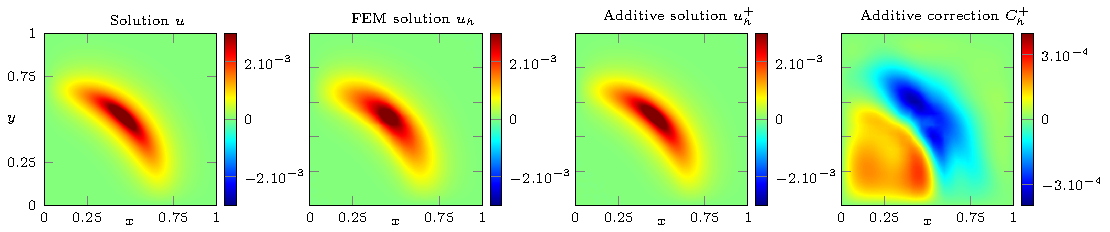
\includegraphics[width=\linewidth]{images/numeric/Anisotropic2D/plots/standalone_solutions.pdf}

	\vspace{4pt}
	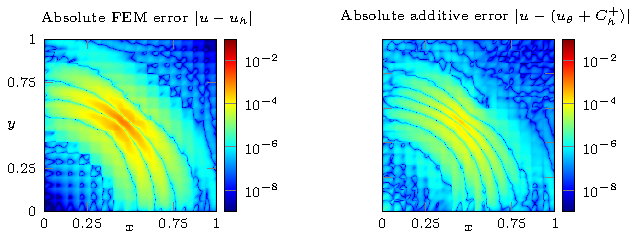
\includegraphics[width=0.5\linewidth]{images/numeric/Anisotropic2D/plots/standalone_errors.pdf}

	\vspace{2pt}
	$\bm{\mu}^{(3)}=(0.46,0.52,0.05,0.12)$ \quad {\small($k=2$, $N=16$)}
\end{frame}

\subsection{Annulus 2D}

\begin{frame}{Poisson on an annulus: problem considered\myfootcite{Sukumar2022}}
	\appendixtarget{annulus}
	\textbf{Test case:} $-\Delta u=f=0$ on $\Omega=\{0.25<\|\bm{x}\|<1\}$, $\bm{\mu}=\mu_1\in[2.4,2.6]$.

	\vspace{-6pt}
	\[
		\left\{
		\begin{aligned}
			u                                       & = g,   &  & \text{on } \Gamma_E \text{ (outer circle)}, \\
			\smash{\frac{\partial u}{\partial n}}+u & = g_R, &  & \text{on } \Gamma_I \text{ (hole)},
		\end{aligned}
		\right.
	\]

	\vspace{4pt}
	\[
		u(\bm{x},\bm{\mu})=1-\frac{\ln\big(\mu_1\|\bm{x}\|\big)}{\ln(4)}, \quad g=1-\frac{\ln(\mu_1)}{\ln(4)}, \quad g_R=2+\frac{4-\ln(\mu_1)}{\ln(4)}
	\]

	\vspace{-4pt}
	\textbf{Parametric PINN:} MLP $5\times 40$, tanh; $4000$ epochs, $6000$ col. pts; \coloredonly<1>{mixed BC exact} + Sobolev training.

	\vspace{6pt}
	\textbf{Boundary conditions depend on $\bm{\mu}$:} harder than the previous cases.
\end{frame}

\begin{frame}{Poisson on an annulus: online phase}
	\setlength{\plotwidth}{0.38\textwidth}\setlength{\plotheight}{0.27\textwidth}
	\begin{minipage}[t]{0.50\linewidth}
		\vspace{0pt}
		{\centering
			\textbf{$L^2$ error, $\bm{\mu}^{(1)}=2.51$}

			\vspace{-2pt}
			\cvgFEMCorrAlldeg{images/numeric/Annulus2D/cvg/FEM_case5_v2_param1.csv}{images/numeric/Annulus2D/cvg/Corr_case5_v2_param1.csv}{1e-10}{false}}
	\end{minipage} \hfill \begin{minipage}[t]{0.46\linewidth}
		\vspace{0pt}
		\only<2->{%
			\small
			\textbf{Gains over FEM:} $\|u-u_h\|_{L^2}/\|u-u_{h,\theta}^+\|_{L^2}$

			\vspace{2pt}
			$N_\mu=50$ parameters, $h=1.33\cdot 10^{-1}$.

			\vspace{4pt}
			\centering
			\GainsTableAlldeg{images/numeric/Annulus2D/gains/Tab_stats_case5_v2_firstN.csv}
		}
	\end{minipage}
\end{frame}

\begin{frame}{Poisson on an annulus: solutions and errors}
	\centering
	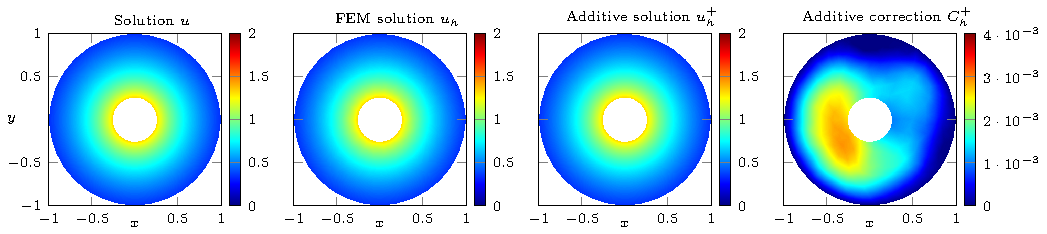
\includegraphics[width=\linewidth]{images/numeric/Annulus2D/plots/standalone_solutions.pdf}

	\vspace{4pt}
	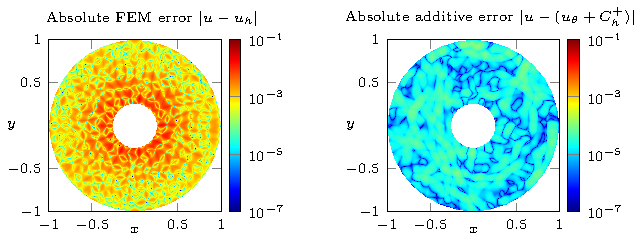
\includegraphics[width=0.5\linewidth]{images/numeric/Annulus2D/plots/standalone_errors.pdf}

	\vspace{2pt}
	$\bm{\mu}^{(1)}=2.51$ \quad {\small($k=1$, $h=1.67\cdot 10^{-1}$)}
\end{frame}
